\documentclass[10pt]{article}
\usepackage{geometry}                % See geometry.pdf to learn the layout options. There are lots.
\geometry{letterpaper}                   % ... or a4paper or a5paper or ... 

\usepackage{enumitem}
\usepackage{graphicx}
\usepackage{subcaption}
%%%%%%%%%%%%%%%%%%%%
\usepackage{mwe}

\title {Deep Learning - HW1}
\author{Afek Adler \& Or Wolkomir}

\begin{document}
\maketitle
\section{Theory}
\subsection{Question 1 - network architecture}
\begin{enumerate}[label=(\alph*)]

\item The input shape is (m,10)
\item $W_h$ shape is $(10,50)$ and $b_h$ shape is $(,50)$
\item $W_o$  shape is $(50,3)$ and $b_0$ shape is $(,3)$
\item y  shape is $(m,3)$
\item $W_h$ shape is $(50,3)$ and $b_h$ shape is $(,3)$
\end{enumerate}

\subsection{Question 2 - \# of parameters}
\begin{enumerate}[label=(\alph*)]

\item \textbf{Conv layer 1} \\
Kernel =  3 \\
Channels = 3 \\
Output = 100 \\
Bias := Output\\
Therefore:\\
\[\#\_of\_parameters = Kernel^{2}*Channels*Output + Bias \Rightarrow \] 
\[3^{3}*100 + 100 = 2,800\] 

\item \textbf{Conv layer 2} \\
Kernel =  3 \\
Channels = 100 \\
Output = 200 \\
Bias := Output\\
Therefore:\\
\[\#\_of\_parameters = Kernel^{2}*Channels*Output + Bias \Rightarrow \] 
\[3^{2}*100*200 +200 = 180,200\] 

\item \textbf{Conv layer3} \\
Kernel =  3 \\
Channels = 200 \\
Output = 400 \\
Bias := Output\\
Therefore:\\
\[\#\_of\_parameters = Kernel^{2}*Channels*Output + Bias \Rightarrow \] 
\[3^{2}*200*400 +400 = 720,400\] 

\item \textbf{Total} \\
\[total\_\#\_of\_parameters = 720,400 + 180,200 +  2,800 = 903,400 \] 
\end{enumerate}

\subsection{Question 3 - deriving BatchNorm  gradients} 
\\
\begin{enumerate}[label=(\alph*)]
\item \textbf{$\frac{\partial f}{\partial \gamma} = $} \\
\begin{equation}
\frac{\partial f}{\partial y} \cdot \frac{\partial y}{\partial \gamma} =\sum_{i=1}^{m} \frac{\partial f}{\partial y_{i}} \cdot \widehat{x}_{i}
\end{equation}

\item \textbf{$\frac{\partial f}{\partial \beta} = $} \\
\begin{equation}
{\frac{\partial f}{\partial y} \cdot \frac{\partial y}{\partial \beta}}
{=\sum_{i=1}^{m} \frac{\partial f}{\partial y_{i}}} 
{\frac{\partial f}{\partial \beta}=\sum_{i=1}^{m} \frac{\partial f}{\partial y_{i}}}
\end{equation}

\item \textbf{$\frac{\partial f}{\partial \widehat{x}_{i}} = $} \\
\begin{equation}
{\frac{\partial f}{\partial y} \cdot \frac{\partial y}{\partial \widehat{x}_{i}}}
{=\frac{\partial f}{\partial y_{i}}} \cdot \gamma
\end{equation}

\item \textbf{$\frac{\partial f}{\partial \sigma^{2}} = $} \\
\begin{equation}
{\frac{\partial f}{\partial \widehat{x}} \cdot \frac{\partial \widehat{x}}{\partial  \sigma^{2}} =
\frac{\partial y}{\partial \widehat{x}_{i}}}
{=\frac{\partial f}{\partial y_{i}}} \cdot \gamma
\end{equation}

\item \textbf{$\frac{\partial f}{\partial \mu} = $} \\
\begin{equation}
\begin{array}{l}{\frac{\partial f}{\partial \mu}=\frac{\partial f}{\partial \hat{x}} \cdot \frac{\partial \hat{x}}{\partial \mu}+\frac{\partial f}{\partial \sigma^{2}} \cdot \frac{\partial \sigma^{2}}{\partial \mu}=} \\ {=\sum_{i=1}^{m} \frac{\partial f}{\partial \hat{x}_{i}} \cdot \frac{\partial \hat{x}_{i}}{\partial \mu}+\frac{\partial f}{\partial \sigma^{2}} \cdot \frac{\partial \sigma^{2}}{\partial \mu}} \\ {\frac{\partial \hat{x}_{i}}{\partial \mu}=\frac{-1}{\sqrt{\sigma^{2}+\epsilon}}} \\ {\frac{\partial \sigma^{2}}{\partial \mu}=-\frac{2}{m} \cdot \sum_{i=1}^{m}\left(x_{i}-\mu\right)} \\ {\frac{\partial f}{\partial \sigma^{2}}=\left(-\frac{1}{2}\right) \cdot \sum_{i=1}^{m} \frac{\partial f}{\partial \hat{x}_{i}} \cdot\left(x_{i}-\mu\right) \cdot\left(\sigma^{2}+\epsilon\right)^{-\frac{3}{2}}}
{\frac{\partial f}{\partial \mu}=\left(\sum_{i=1}^{m} \frac{\partial f}{\partial \hat{x}_{i}} \cdot \frac{\partial \hat{x}_{i}}{\partial \mu}\right)+\left(\frac{\partial f}{\partial \sigma^{2}} \cdot \frac{\partial \sigma^{2}}{\partial \mu}\right)=} \\ {=\left(\sum_{i=1}^{m} \frac{\partial f}{\partial \hat{x}_{i}} \cdot \frac{-1}{\sqrt{\sigma^{2}+\epsilon}}\right)+\left(\frac{\partial f}{\partial \sigma^{2}} \cdot\left(-\frac{2}{m}\right) \cdot \sum_{i=1}^{m}\left(x_{i}-\mu\right)\right)=} \\ {=\sum_{i=1}^{m} \frac{\partial f}{\partial \hat{x}_{i}} \cdot \frac{-1}{\sqrt{\sigma^{2}+\epsilon}}+\frac{\partial f}{\partial \sigma^{2}} \cdot\left(-\frac{2}{m}\right)  \cdot\left[\sum_{i=1}^{m}\left(x_{i}\right)-\sum_{i=1}^{m}(\mu)\right]} {=\sum_{i=1}^{m} \frac{\partial f}{\partial \hat{x}_{i}} \cdot \frac{-1}{\sqrt{\sigma^{2}+\epsilon}}\\+\frac{\partial f}{\partial \sigma^{2}} \cdot(-2) \cdot\left[\frac{1}{m} \sum_{i=1}^{m}\left(x_{i}\right)-\frac{1}{m} \sum_{i=1}^{m}(\mu)\right]=}
{=\sum_{i=1}^{m} \frac{\partial f}{\partial \hat{x}_{i}} \cdot \frac{-1}{\sqrt{\sigma^{2}+\epsilon}}+\frac{\partial f}{\partial \sigma^{2}} \cdot(-2) \cdot\left[\mu-\frac{1}{m} \sum_{i=1}^{m} \mu\right]=} \\ {=\sum_{i=1}^{m} \frac{\partial f}{\partial \hat{x}_{i}} \cdot \frac{-1}{\sqrt{\sigma^{2}+\epsilon}}+\frac{\partial f}{\partial \sigma^{2}} \cdot(-2) \cdot\left[\mu-\frac{1}{m} \cdot m \cdot \mu\right]=} \\ {=\sum_{i=1}^{m} \frac{\partial f}{\partial \hat{x}_{i}} \cdot \frac{-1}{\sqrt{\sigma^{2}+\epsilon}}+\frac{\partial f}{\partial \sigma^{2}} \cdot 0=} \\ {=\sum_{i=1}^{m} \frac{\partial f}{\partial \hat{x}_{i}} \cdot \frac{-1}{\sqrt{\sigma^{2}+\epsilon}}}\end{array}
\end{equation}




\item \textbf{$\frac{\partial f}{\partial x_i} = $} \\
\begin{equation}
\begin{array}{l}
\frac{\partial f}{\partial x_{i}}=\frac{\partial f}{\partial \hat{x}_{i}} \cdot \frac{\partial \hat{x}_{i}}{\partial x_{i}}+\frac{\partial f}{\partial \mu} \cdot \frac{\partial \mu}{\partial x_{i}}+\frac{\partial f}{\partial \sigma^{2}} \cdot \frac{\partial \sigma^{2}}{\partial x_{i}}= \\
{\frac{\partial \hat{x}_{i}}{\partial x_{i}}=\frac{1}{\sqrt{\sigma^{2}+\epsilon}}} \\
{\frac{\partial \mu}{\partial x_{i}}=\frac{1}{m}} \\ {\frac{\partial \sigma^{2}}{\partial x_{i}}=\frac{2}{m} \cdot\left(x_{i}-\mu\right)}
{\frac{\partial f}{\partial x_{i}}=\frac{\partial f}{\partial \hat{x}_{i}} \cdot \frac{\partial \hat{x}_{i}}{\partial x_{i}}+\frac{\partial f}{\partial \mu} \cdot \frac{\partial \mu}{\partial x_{i}}+\frac{\partial f}{\partial \sigma^{2}} \cdot \frac{\partial \sigma^{2}}{\partial x_{i}}=} \\ {=\left(\frac{\partial f}{\partial \hat{x}_{i}} \cdot \frac{1}{\sqrt{\sigma^{2}+\epsilon}}\right)+\left(\frac{\partial f}{\partial \mu} \cdot \frac{1}{m}\right)+\left(\frac{\partial f}{\partial \sigma^{2}} \cdot \frac{2}{m}\left(x_{i}-\mu\right)\right)=} \\ {=\left(\frac{\partial f}{\partial \hat{x}_{i}} \cdot \frac{1}{\sqrt{\sigma^{2}+\epsilon}}\right)+\left(\frac{1}{m} \cdot \sum_{i=1}^{m} \frac{\partial f}{\partial \hat{x}_{i}} \cdot \frac{-1}{\sqrt{\sigma^{2}+\epsilon}}\right)+\left(\frac{\partial f}{\partial \sigma^{2}} \cdot \frac{2}{m}\left(x_{i}-\mu\right)\right)=}\\ 
{\left(\frac{\partial f}{\partial \hat{x}_{i}} \cdot \frac{1}{\sqrt{\sigma^{2}+\epsilon}}\right)+\left(\frac{1}{m} \cdot \sum_{i=1}^{m} \frac{\partial f}{\partial \hat{x}_{i}} \cdot \frac{-1}{\sqrt{\sigma^{2}+\epsilon}}\right)+ \left(\left[\left(-\frac{1}{2}\right) \cdot \sum_{j=1}^{m} \frac{\partial f}{\partial \hat{x}_{j}} \cdot\left(x_{j}-\mu\right) \cdot\left(\sigma^{2}+\epsilon\right)^{-\frac{3}{2}}\right] \cdot \frac{2}{m}\left(x_{i}-\mu\right)\right)} \\ {=\left(\frac{\partial f}{\partial \hat{x}_{i}} \cdot \frac{1}{\sqrt{\sigma^{2}+\epsilon}}\right)+\left(\frac{1}{m} \cdot \sum_{i=1}^{m} \frac{\partial f}{\partial \hat{x}_{i}} \cdot  \frac{-1}{\sqrt{\sigma^{2}+\epsilon}}\right)+\left(-\left[\frac{1}{m} \cdot \sum_{j=1}^{m} \frac{\left(x_{j}-\mu\right)}{\sqrt{\sigma^{2}+\epsilon}} \cdot\left(\sigma^{2}+\epsilon\right)^{-1} \frac{\partial f}{\partial \hat{x}_{j}}\right] \cdot\left(x_{i}-\mu\right)\right)} \\ {=\left(\frac{\partial f}{\partial \hat{x}_{i}} \cdot \frac{1}{\sqrt{\sigma^{2}+\epsilon}}\right)+\left(\frac{1}{m} \cdot \sum_{i=1}^{m} \frac{\partial f}{\partial \hat{x}_{i}} \cdot \frac{-1}{\sqrt{\sigma^{2}+\epsilon}}\right)+\left(-\left[\frac{1}{m} \cdot \sum_{j=1}^{m} \frac{\left(x_{j}-\mu\right)}{\sqrt{\sigma^{2}+\epsilon}} \frac{\partial f}{\partial \hat{x}_{j}} \cdot\left(\sigma^{2}+\epsilon\right)^{-\frac{1}{2}}\right] \cdot \frac{\left(x_{i}-\mu\right)}{\sqrt{\sigma^{2}+\epsilon}}\right)}\\
{=\left(\frac{\partial f}{\partial \hat{x}_{i}} \cdot \frac{1}{\sqrt{\sigma^{2}+\epsilon}}\right)+\left(\frac{1}{m} \cdot \sum_{i=1}^{m} \frac{\partial f}{\partial \hat{x}_{i}} \cdot \frac{-1}{\sqrt{\sigma^{2}+\epsilon}}\right)+\left(-\left[\frac{1}{m} \cdot \sum_{j=1}^{m} \hat{x}_{j} \cdot \frac{\partial f}{\partial \hat{x}_{j}} \cdot\left(\sigma^{2}+\epsilon\right)^{-\frac{1}{2}}\right] \cdot \hat{x}_{i}\right)} \\ {=\left(\frac{\partial f}{\partial \hat{x}_{i}} \cdot \frac{1}{\sqrt{\sigma^{2}+\epsilon}}\right)+\left(\frac{1}{m} \cdot \sum_{i=1}^{m} \frac{\partial f}{\partial \hat{x}_{i}} \cdot \frac{-1}{\sqrt{\sigma^{2}+\epsilon}}\right)+\left(-\frac{1}{m \cdot \sqrt{\sigma^{2}+\epsilon}} \cdot \sum_{j=1}^{m}\left(\hat{x}_{j} \cdot \frac{\partial f}{\partial \hat{x}_{j}}\right) \cdot \hat{x}_{i}\right)} \\ {=\frac{1}{\sqrt{\sigma^{2}+\epsilon}} \cdot\left[\frac{\partial f}{\partial \hat{x}_{i}}-\frac{1}{m} \sum_{i=1}^{m} \frac{\partial f}{\partial \hat{x}_{i}}-\frac{\hat{x}_{i}}{m} \sum_{j=1}^{m}\left(\hat{\chi}_{j} \cdot \frac{\partial f}{\partial \hat{x}_{j}}\right)\right]}
\end{array}
\end{equation}
\end{enumerate}

% 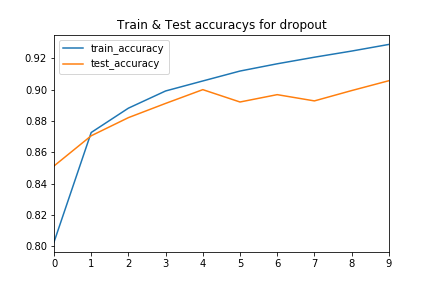
\includegraphics[height = 3cm]{figures/dropout}
\newpage 

\section{Practical}
We wanted to compare apples to apples so we tried to keep most hyper-parameters consistent across experiments, for educational purposes (it is clear that if we would do grid search for example most likely that hyper-parameters will vary between experiments).
As well, we would like to note that we did no perform hyper-parameter tuning, because the networks achieved sufficient performance out of the box. This is way we also did not use a validation data set.\\
As we wanted to compare apples to apples we regularized the model only in one layer, after the first fully connected layer. We could have also done differently (another hyper-parameter).
We used the following hyper-parameters across all the experiments :
\begin{enumerate}[label=(\alph*)]
\item Optimizer - ADAM with default $\beta_1$ and $\beta_2$
\item Learning rate - 0.001
\item Epochs - 10. We would like to note that we set seed for each experiment, so if it was a real model (in production), we can perform early stopping and choose the best score. But than it's better to do have a test score as well (because we are "playing" with the model) in order to get a real estimate about the algorithm accuracy. 
\end{enumerate}

Hyper-parameters that are unique for each experiment - 
\begin{enumerate}[]
\item BatchNorm with hyper-paramerter affine = False
\item Dropout (with 10%)
\item Weight decay (for all weights, not only one layer) - $2 \cdot 10^{-4}$
\item No regularization
\end{enumerate}

Conclusions
\begin{enumerate}[label=(\alph*)]
\item For all the experiments after 2-3 epochs the model over-fits. 
\item Even though over-fitting happens validation scores keep increasing with the epochs. 
\item All the models are pretty much the same (around 90\% accuracy). So in order to argue which model is better it's better to perform an hypothesis test.
\end{enumerate}

\newpage 
\subsection{Graphs}
% \subsection{Graphs}
% \begin{figure}[ht]
% \centering
% \begin{subfigure}{.2\textwidth}
%     \centering
%     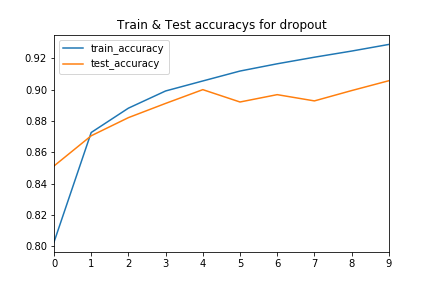
\includegraphics[0.5]{figures/dropout}
% \end{subfigure}%
% \begin{subfigure}{.2\textwidth}
%     \centering
%     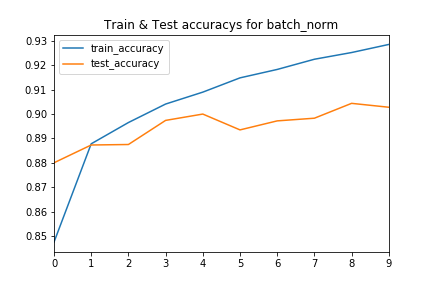
\includegraphics[0.5]{figures/batch_norm}
% \end{subfigure}
% \begin{subfigure}{.2\textwidth}
%     \centering
%     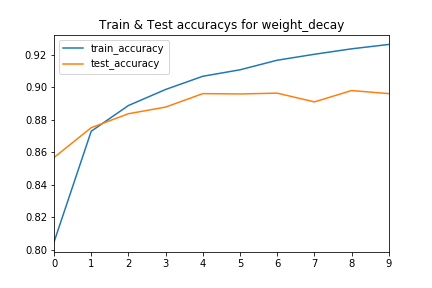
\includegraphics[0.5]{figures/weight_decay}
% \end{subfigure}%
% \begin{subfigure}{.2\textwidth}
%     \centering
%     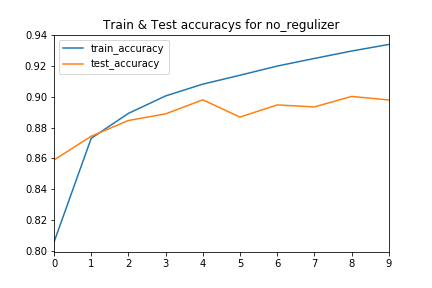
\includegraphics[0.5]{figures/no_regulizer}
% \end{subfigure}
% \caption[short]{}
% \end{figure}

    \begin{figure*}[ht]
        \centering
        \begin{subfigure}[b]{0.475\textwidth}
            \centering
            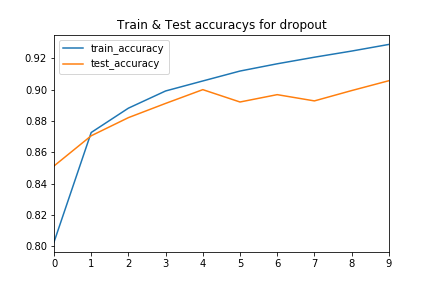
\includegraphics[width=\textwidth]{figures/dropout}
            \caption[Network2]%
            {{\small }}    
            \label{fig:mean and std of net14}
        \end{subfigure}
        \hfill
        \begin{subfigure}[b]{0.475\textwidth}  
            \centering 
            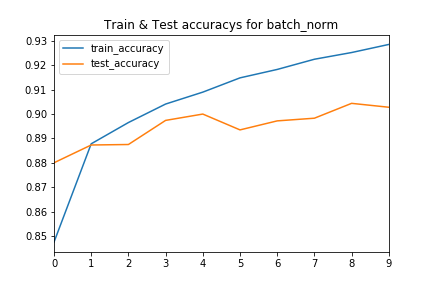
\includegraphics[width=\textwidth]{figures/batch_norm}
            \caption[]%
            {{\small}}    
            \label{fig:mean and std of net24}
        \end{subfigure}
        \vskip\baselineskip
        \begin{subfigure}[b]{0.475\textwidth}   
            \centering 
            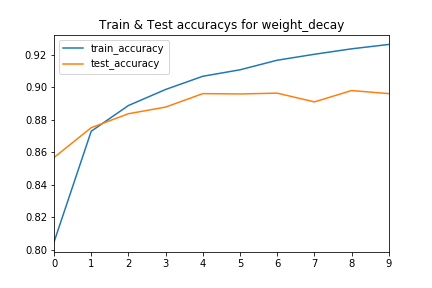
\includegraphics[width=\textwidth]{figures/weight_decay}
            \caption[]%
            {{\small 3}}    
            \label{fig:mean and std of net34}
        \end{subfigure}
        \quad
        \begin{subfigure}[b]{0.475\textwidth}   
            \centering 
            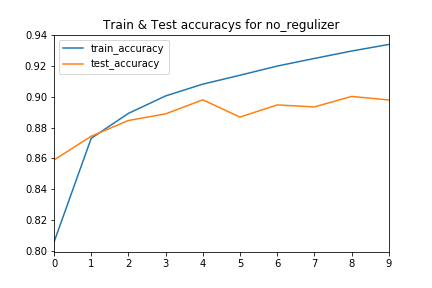
\includegraphics[width=\textwidth]{figures/no_regulizer}
            \caption[]%
            {{\small}}    
            \label{fig:mean and std of net44}
        \end{subfigure}
        \caption[ The average and standard deviation of critical parameter ]
        {\small Convergence graphs} 
        \label{fig:mean and std of nets}
    \end{figure*}


\end{document}  
